\documentclass[conference]{IEEEtran}

\usepackage{amsmath,amssymb,amsfonts}
\usepackage{graphicx}
\usepackage{textcomp}
\usepackage{booktabs}
\usepackage{multirow}
\usepackage{algorithm}
\usepackage{algorithmic}
\usepackage{hyperref}
\usepackage{xcolor}
\usepackage{array}
\usepackage{bm}
\usepackage{mathtools}
\usepackage{enumitem}

% Shorthand commands
\newcommand{\R}{\mathbb{R}}
\newcommand{\N}{\mathcal{N}}
\newcommand{\E}{\mathcal{E}}
\newcommand{\V}{\mathcal{V}}
\newcommand{\Loss}{\mathcal{L}}
\newcommand{\vect}[1]{\bm{#1}}
\newcommand{\mat}[1]{\mathbf{#1}}
\DeclareMathOperator{\sigmoid}{sigmoid}
\DeclareMathOperator{\softmax}{softmax}
\DeclareMathOperator{\ReLU}{ReLU}
\DeclareMathOperator{\LN}{LayerNorm}
\DeclareMathOperator{\BN}{BatchNorm}
\DeclareMathOperator{\BCE}{BCE}
\DeclareMathOperator{\CE}{CE}

\begin{document}

\title{A Complete Theoretical and Practical Guide to\\LSGNN-DualTask for Network Intrusion Detection:\\From Raw Packets to Graph Neural Network Classification}

\author{
\IEEEauthorblockN{Author One\IEEEauthorrefmark{1}, Author Two\IEEEauthorrefmark{1}, Author Three\IEEEauthorrefmark{1}}
\IEEEauthorblockA{\IEEEauthorrefmark{1}Department of Computer Science\\
University Placeholder, City, Country\\
\{author.one, author.two, author.three\}@university.edu}
}

\maketitle

\begin{abstract}
This report provides a complete, self-contained theoretical and practical walkthrough of our end-to-end pipeline for network intrusion detection using Graph Neural Networks. Starting from raw packet capture data with only 9~columns, we explain every mathematical transformation applied: feature engineering (deriving 68~features from sparse data), graph construction (k-nearest-neighbor similarity and communication-pattern edges), the Local Similarity Graph Neural Network (LSGNN) architecture with its similarity-weighted message passing, and our novel extension---LSGNN-DualTask---which adds an edge consistency regularization loss. For each component, we present the exact mathematical formulation, explain the intuition behind it, and describe the code-level implementation. We also cover SMOTE-based data augmentation, inverse-frequency class weighting, cosine annealing with warmup, label smoothing, and all training details. This report is intended as a learning document: every equation is explained step by step, every design choice is justified, and the full experimental results are analyzed.
\end{abstract}

\begin{IEEEkeywords}
Graph Neural Networks, LSGNN, Dual-Task Learning, Edge Consistency, Network Intrusion Detection, Feature Engineering, SMOTE, Message Passing
\end{IEEEkeywords}

% ======================================================================
\section{Introduction: What Are We Trying to Do?}
% ======================================================================

Our goal is to classify network packets into one of five traffic categories:

\begin{enumerate}[leftmargin=2em]
    \item \textbf{BENIGNE}: Normal, legitimate traffic (23.5\%).
    \item \textbf{Copy 54ndc47 (SMB)}: An SMB-based file copy attack (68.7\%).
    \item \textbf{Service Creation}: Remote service creation for persistence (4.3\%).
    \item \textbf{Discover local hosts}: Network scanning/discovery (3.4\%).
    \item \textbf{View remote shares}: SMB share enumeration (0.1\%).
\end{enumerate}

The challenge is that our raw data has only 9~columns (\texttt{packet\_id}, \texttt{timestamp}, \texttt{label}, \texttt{src\_ip}, \texttt{dst\_ip}, \texttt{protocol}, \texttt{src\_port}, \texttt{dst\_port}, \texttt{length}), the classes are extremely imbalanced (713:1 ratio), and the attacks represent sequential stages of a lateral movement campaign. We tackle this with a pipeline that has six stages, each building on the previous one.

\begin{figure}[t]
    \centering
    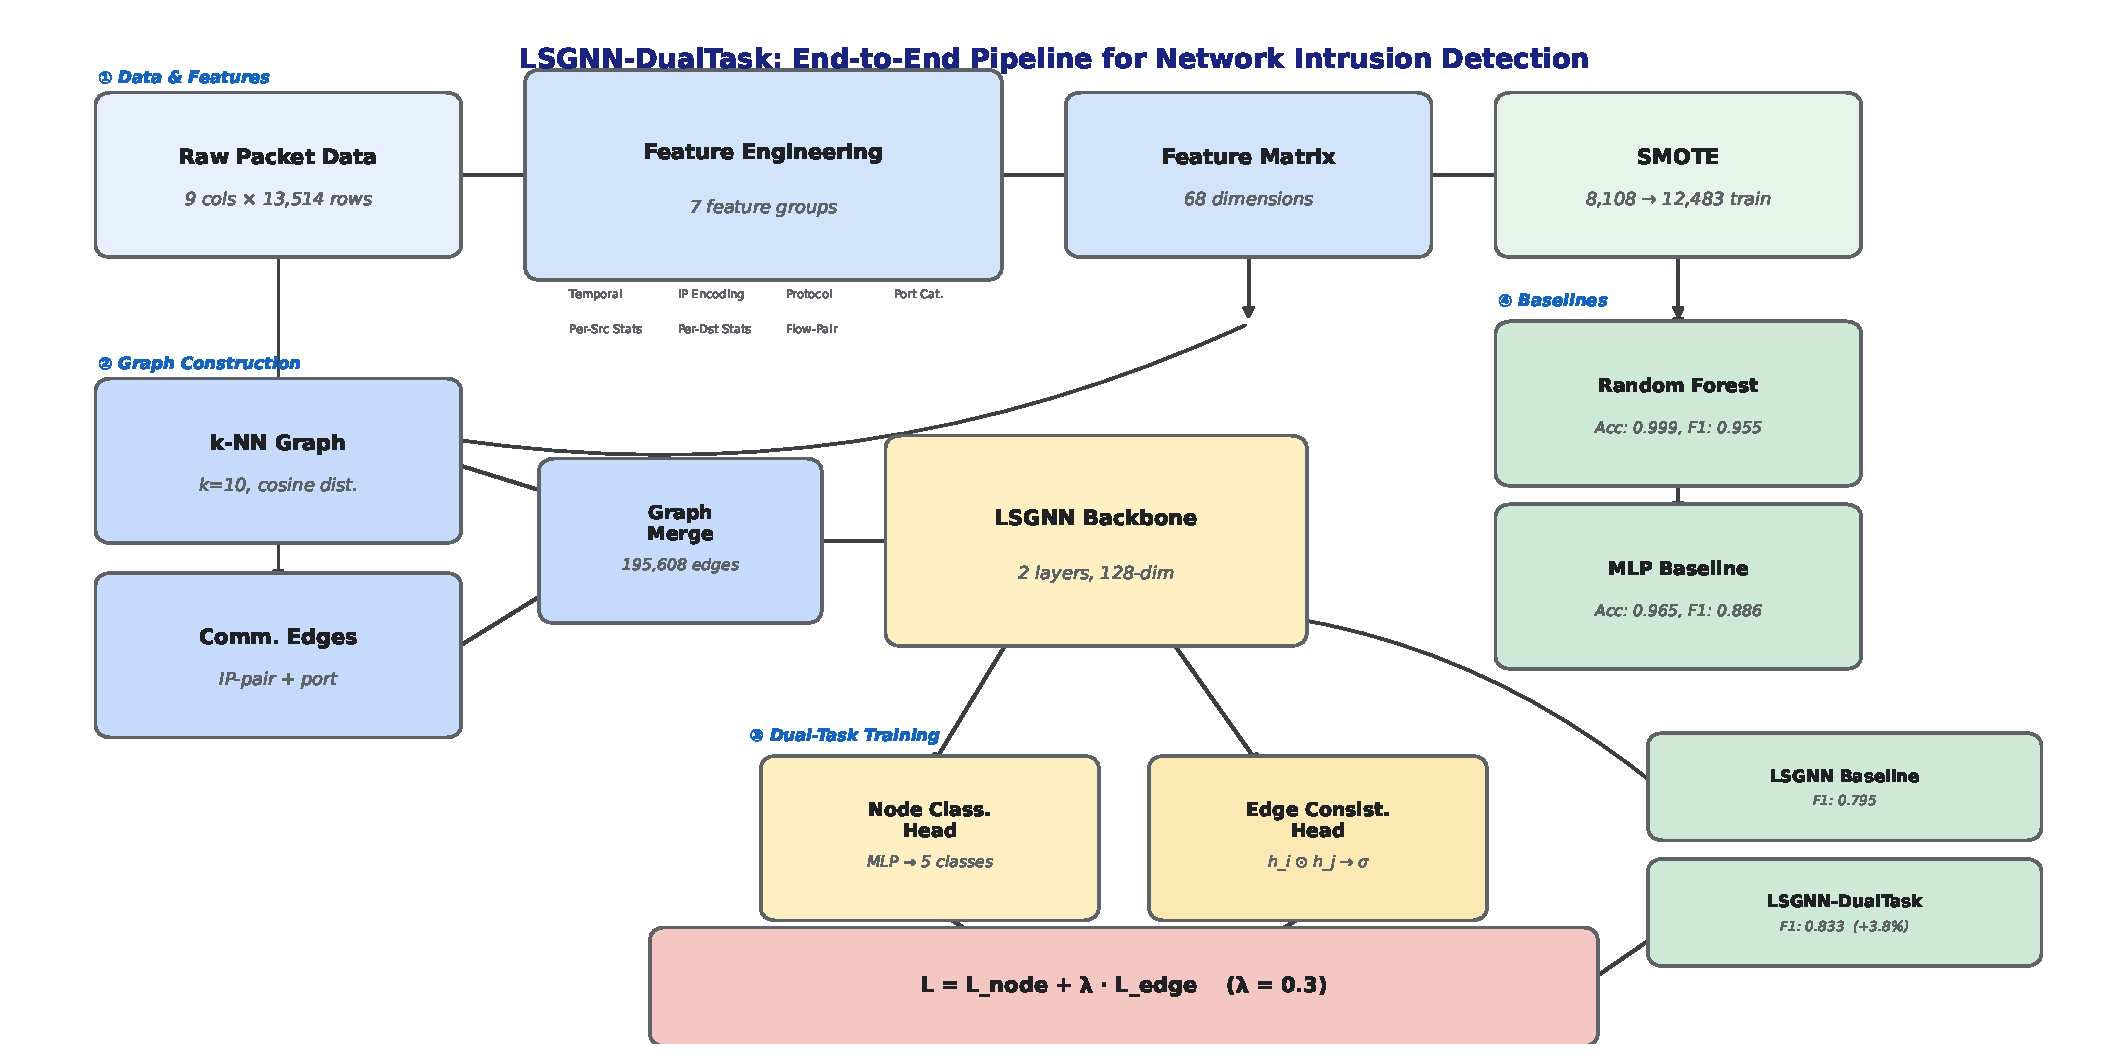
\includegraphics[width=\columnwidth]{figures/pipeline.pdf}
    \caption{Overview of the complete pipeline. Each numbered stage is explained in its own section of this report.}
    \label{fig:pipeline}
\end{figure}

% ======================================================================
\section{Stage 1: Feature Engineering}
\label{sec:features}
% ======================================================================

\subsection{Why Feature Engineering Matters Here}

With only 9~raw columns, a classifier has very little signal. An IP address like ``192.168.10.100'' is a string---a model cannot use it directly. A single port number like 445 is just a number without context. Feature engineering creates \emph{meaningful numeric representations} from this sparse data. We derive 68~features organized into seven groups.

\subsection{Group 1: Packet-Level Features (14 features)}

These are direct transformations of the raw per-packet values.

\textbf{Length and log-length.} Packet length $\ell_i$ is kept as-is, and we also compute:
\begin{equation}
    \text{length\_log}_i = \log(1 + \ell_i)
\end{equation}
The $\log(1 + x)$ transform (called \texttt{log1p}) compresses large values and reduces the impact of very large packets. This helps because packet lengths span from 54 to 1514 bytes, and the distribution is skewed.

\textbf{Port category indicators.} Port numbers are divided into three IANA-defined ranges:
\begin{align}
    \text{wellknown}_i &= \mathbb{1}[\text{port}_i < 1024] \\
    \text{registered}_i &= \mathbb{1}[1024 \leq \text{port}_i < 49152] \\
    \text{dynamic}_i &= \mathbb{1}[\text{port}_i \geq 49152]
\end{align}
where $\mathbb{1}[\cdot]$ is the indicator function (returns 1 if true, 0 if false). This is done separately for source and destination ports, yielding 6~features. The intuition is that well-known ports indicate standard services (HTTP, SMB), while dynamic ports indicate ephemeral client connections.

\textbf{Key service port flags.} For specific ports known to be attack-relevant:
\begin{equation}
    \text{dst\_port\_is\_}p_i = \mathbb{1}[\text{dst\_port}_i = p], \quad p \in \{80, 443, 445, 135, 21, 53\}
\end{equation}
Port 445 (SMB) is especially important since the dominant attack uses it.

\textbf{Same-port indicator:}
\begin{equation}
    \text{same\_port}_i = \mathbb{1}[\text{src\_port}_i = \text{dst\_port}_i]
\end{equation}

\subsection{Group 2: Protocol One-Hot Encoding (4 features)}

The protocol field takes values 6 (TCP), 17 (UDP), 1 (ICMP), or is missing. Instead of using the raw number (which would imply an ordering: ``TCP $<$ UDP''), we create binary indicators:
\begin{align}
    \text{proto\_tcp}_i &= \mathbb{1}[\text{protocol}_i = 6] \\
    \text{proto\_udp}_i &= \mathbb{1}[\text{protocol}_i = 17] \\
    \text{proto\_icmp}_i &= \mathbb{1}[\text{protocol}_i = 1] \\
    \text{proto\_missing}_i &= \mathbb{1}[\text{protocol}_i = \text{NaN}]
\end{align}
This is called \emph{one-hot encoding}: each category becomes its own binary feature. It works because protocols are \emph{categorical}---there is no meaningful ``distance'' between TCP and UDP.

\subsection{Group 3: IP Address Encoding (12 features)}

IP addresses like ``192.168.10.100'' are strings. We extract each octet as a separate numeric feature. For an IP address $a.b.c.d$:
\begin{equation}
    \text{ip\_oct0} = a, \quad \text{ip\_oct1} = b, \quad \text{ip\_oct2} = c, \quad \text{ip\_oct3} = d
\end{equation}
This gives 4~features each for source and destination (8~total). We also compute:
\begin{align}
    \text{same\_subnet\_16}_i &= \mathbb{1}[\text{src\_oct0} = \text{dst\_oct0} \;\wedge\; \text{src\_oct1} = \text{dst\_oct1}] \\
    \text{same\_subnet\_24}_i &= \text{same\_subnet\_16}_i \;\wedge\; \mathbb{1}[\text{src\_oct2} = \text{dst\_oct2}]
\end{align}
and flags for missing IPs, internal IPs ($192.168.x.x$ or $10.x.x.x$), and whether both endpoints are internal.

\subsection{Group 4: Temporal Features (11 features)}

The dataset is sorted by timestamp $t_i$. We compute:

\textbf{Relative time:}
\begin{equation}
    \tau_i = t_i - t_{\min}, \quad \hat{\tau}_i = \frac{t_i - t_{\min}}{t_{\max} - t_{\min}}
\end{equation}

\textbf{Inter-arrival time (IAT):} The time between consecutive packets:
\begin{equation}
    \Delta t_i = t_i - t_{i-1}, \quad \Delta t_0 = 0
\end{equation}
This is critical: bursts of rapid packets (very small $\Delta t$) often indicate automated attacks, while normal traffic has more variable timing.

\textbf{Burst detection:}
\begin{equation}
    \text{is\_burst}_i = \mathbb{1}[\Delta t_i < 0.001 \text{ sec}]
\end{equation}

\textbf{Rolling window statistics.} For windows of size $w \in \{10, 50\}$:
\begin{align}
    \text{iat\_mean}_{w,i} &= \frac{1}{\min(i+1, w)} \sum_{j=\max(0, i-w+1)}^{i} \Delta t_j \\
    \text{iat\_std}_{w,i} &= \sqrt{\frac{1}{\min(i+1,w)} \sum_{j} (\Delta t_j - \text{iat\_mean}_{w,i})^2}
\end{align}
and similarly for packet length. These capture local traffic patterns: a sudden change in mean IAT or packet size within a window indicates a shift in traffic behavior.

\subsection{Group 5: Per-Source Statistics (7 features)}

These aggregate information across all packets from the same source IP:

\textbf{Source frequency (frequency encoding):}
\begin{equation}
    \text{src\_ip\_freq}_i = \frac{|\{j : \text{src\_ip}_j = \text{src\_ip}_i\}|}{N}
\end{equation}
where $N$ is the total number of packets. This replaces the categorical IP string with a numeric value capturing ``how active is this source?''

\textbf{Average length per source:}
\begin{equation}
    \text{src\_avg\_length}_i = \frac{1}{|\{j : \text{src\_ip}_j = \text{src\_ip}_i\}|} \sum_{\{j : \text{src}_j = \text{src}_i\}} \ell_j
\end{equation}

\textbf{Unique destinations and ports:}
\begin{equation}
    \text{src\_unique\_dsts}_i = |\{\text{dst\_ip}_j : \text{src\_ip}_j = \text{src\_ip}_i\}|
\end{equation}
A source contacting many destinations may be performing a network scan.

\textbf{Port entropy (scanning detection):}
\begin{equation}
    H_{\text{port}}(\text{src}_i) = - \sum_{p} \hat{f}_p \log_2 \hat{f}_p
\end{equation}
where $\hat{f}_p$ is the fraction of packets from $\text{src}_i$ targeting port $p$. High entropy means the source uses many different ports---a strong indicator of scanning behavior.

\textbf{Packet and byte rates:}
\begin{equation}
    \text{src\_packet\_rate}_i = \frac{n_{\text{src}_i}}{t^{\text{last}}_{\text{src}_i} - t^{\text{first}}_{\text{src}_i} + \epsilon}
\end{equation}
where $\epsilon = 10^{-6}$ prevents division by zero.

\subsection{Group 6: Per-Destination Statistics (3 features)}

Analogous to Group~5 but aggregated per destination IP: frequency, average length, and unique source count.

\subsection{Group 7: Flow-Pair and Advanced Features (21 features)}

\textbf{IP pair frequency:}
\begin{equation}
    \text{pair\_freq}_i = \frac{|\{j : \text{src}_j \to \text{dst}_j = \text{src}_i \to \text{dst}_i\}|}{N}
\end{equation}

\textbf{Reverse flow indicator:}
\begin{equation}
    \text{has\_reverse}_i = \mathbb{1}[\exists\, j : \text{src}_j = \text{dst}_i \;\wedge\; \text{dst}_j = \text{src}_i]
\end{equation}
Bidirectional communication is more typical of legitimate traffic, while unidirectional flows may indicate scanning or exfiltration.

\textbf{Sliding-window source packet counts.} For windows $w \in \{10, 50, 100\}$:
\begin{equation}
    \text{src\_pkt\_count}_{w,i} = |\{j : \max(0, i-w) \leq j \leq i,\; \text{src}_j = \text{src}_i\}|
\end{equation}
This captures how active a source is in the recent local context.

\subsection{Standardization}

After computing all 68~features, we standardize each feature to zero mean and unit variance:
\begin{equation}
    \hat{x}^{(k)}_i = \frac{x^{(k)}_i - \mu_k}{\sigma_k}
\end{equation}
where $\mu_k$ and $\sigma_k$ are the mean and standard deviation of feature $k$ across all samples. This is critical because features have very different scales (e.g., port numbers range 0--65535, while frequencies are in $[0,1]$), and most ML models (especially neural networks) work best when features are on similar scales.

% ======================================================================
\section{Stage 2: Handling Class Imbalance with SMOTE}
\label{sec:smote}
% ======================================================================

\subsection{The Problem}

Our dataset has 9{,}281 samples of the majority class but only 13 of the rarest class. A model that always predicts ``Copy 54ndc47 (SMB)'' would achieve 68.7\% accuracy but would completely fail to detect rare attacks. This is called \emph{class imbalance}.

\subsection{SMOTE: Synthetic Minority Oversampling Technique}

SMOTE~\cite{chawla2002smote} generates new synthetic samples for minority classes. For each minority sample $\vect{x}_i$:

\begin{enumerate}
    \item Find its $k$ nearest neighbors in feature space among the same class (we use $k=5$).
    \item Randomly select one neighbor $\vect{x}_j$.
    \item Create a new synthetic sample by interpolation:
    \begin{equation}
        \vect{x}_{\text{new}} = \vect{x}_i + \alpha \cdot (\vect{x}_j - \vect{x}_i)
    \end{equation}
    where $\alpha \sim \text{Uniform}(0, 1)$.
\end{enumerate}

Geometrically, the new sample is a random point on the line segment between $\vect{x}_i$ and $\vect{x}_j$ in feature space. This creates \emph{novel but realistic} samples rather than simply duplicating existing ones.

\subsection{Handling Very Rare Classes}

For ``View remote shares'' with only 8~training samples, SMOTE cannot work directly because it needs $k+1 = 6$ same-class neighbors. Our solution is a two-step approach:

\begin{enumerate}
    \item \textbf{Step 1 -- RandomOverSampler}: Duplicate samples of tiny classes (with replacement) until each class has at least 6 samples.
    \item \textbf{Step 2 -- SMOTE}: Apply SMOTE targeting 30\% of the majority class count for each minority class.
\end{enumerate}

This augments the training set from 8{,}108 to 12{,}483 samples. Importantly, \emph{only the training set is augmented}---validation and test sets remain untouched to ensure unbiased evaluation.

\subsection{Class Weights (Complementary Strategy)}

In addition to SMOTE, we apply \emph{inverse-frequency class weights} to the loss function. For class $c$ with $n_c$ training samples out of $N$ total:
\begin{equation}
    w_c = \frac{N}{C \cdot n_c}
\end{equation}
where $C$ is the number of classes. We clip weights to $[0.1, 10.0]$ to prevent numerical instability. The cross-entropy loss becomes:
\begin{equation}
    \Loss_{\CE} = -\frac{1}{|\mathcal{S}|} \sum_{i \in \mathcal{S}} w_{y_i} \log \hat{p}_i(y_i)
\end{equation}
where $\mathcal{S}$ is the set of supervised nodes, $y_i$ is the true label, and $\hat{p}_i(y_i)$ is the predicted probability for the correct class. This means a misclassification of a rare class costs more than a misclassification of a common class.

% ======================================================================
\section{Stage 3: Graph Construction}
\label{sec:graph}
% ======================================================================

\subsection{Why Build a Graph?}

Traditional models (Random Forest, MLP) treat each packet independently. But network traffic has natural \emph{relational structure}: packets from the same source, targeting the same service, or occurring in the same time window are related. A graph encodes these relationships, and a Graph Neural Network can then propagate information along edges---if one packet in a flow is suspicious, the GNN can ``spread'' that suspicion to related packets.

Formally, we construct a graph $G = (\V, \E)$ where:
\begin{itemize}
    \item $\V = \{v_1, \ldots, v_N\}$ --- each node $v_i$ is a network packet.
    \item $\E \subseteq \V \times \V$ --- edges connect ``related'' packets.
    \item Each node carries a feature vector $\vect{x}_i \in \R^{68}$.
    \item Each node has a label $y_i \in \{0, 1, 2, 3, 4\}$.
\end{itemize}

\subsection{k-Nearest Neighbor (k-NN) Edges}

For each node $v_i$, we find the $k = 10$ most similar nodes based on cosine distance in feature space:
\begin{equation}
    d_{\cos}(\vect{x}_i, \vect{x}_j) = 1 - \frac{\vect{x}_i \cdot \vect{x}_j}{\|\vect{x}_i\| \cdot \|\vect{x}_j\|}
\end{equation}

The $k$ nodes with smallest cosine distance become neighbors. We symmetrize the graph (if $i$ is a neighbor of $j$, then $j$ is also a neighbor of $i$), resulting in an undirected graph.

\textbf{Intuition}: Packets with similar feature profiles (similar packet size distributions, timing patterns, port usage) are likely the same type of traffic. The k-NN graph encodes this inductive bias.

In our dataset, k-NN produces 177{,}346 edges.

\subsection{Communication-Based Edges}

We add edges based on real network communication patterns:

\textbf{IP-pair edges}: All packets sharing the same (src\_ip, dst\_ip) pair are connected. For small groups ($\leq 100$ packets), each packet connects to the next 4~packets in the group. For large groups ($> 100$), we use a chain topology (each packet connects to the next) to limit density.

\textbf{Port-based edges}: Packets targeting the same destination port are connected (for groups of 2--50 packets, connecting each to the next 2).

This adds 28{,}276 edges. After merging and deduplication, the total graph has \textbf{195{,}608 edges} with average degree 14.5.

\subsection{Edge Homophily}

We measure \emph{edge homophily}: the fraction of edges connecting same-class nodes:
\begin{equation}
    h = \frac{|\{(i,j) \in \E : y_i = y_j\}|}{|\E|}
\end{equation}
Our graph has $h = 0.962$, meaning 96.2\% of edges connect same-class nodes. This is \emph{homophilic}, which means GNNs can leverage the neighbor structure effectively: a node's neighbors are likely the same class, so message passing can reinforce correct predictions.

% ======================================================================
\section{Stage 4: The LSGNN Architecture}
\label{sec:lsgnn}
% ======================================================================

\subsection{Overview}

The Local Similarity Graph Neural Network (LSGNN) is a GNN designed to work on both homophilic and heterophilic graphs. Its key innovation is a \emph{learned similarity score} on each edge that adaptively weights neighbor messages.

The full architecture is:
\begin{equation}
    \text{Input } \vect{x}_i \xrightarrow{\text{Project}} \vect{h}_i^{(0)} \xrightarrow{\text{LSGNN Layer 1}} \vect{h}_i^{(1)} \xrightarrow{\text{LSGNN Layer 2}} \vect{h}_i^{(2)} \xrightarrow{\text{Classifier}} \hat{\vect{y}}_i
\end{equation}

\subsection{Step 1: Input Projection}

The raw 68-dimensional feature vector is projected into a $d_h = 128$ dimensional hidden space:
\begin{equation}
    \vect{h}_i^{(0)} = \text{Dropout}\Big(\ReLU\big(\LN(\mat{W}_{\text{proj}} \vect{x}_i + \vect{b}_{\text{proj}})\big)\Big)
\end{equation}
where:
\begin{itemize}
    \item $\mat{W}_{\text{proj}} \in \R^{128 \times 68}$ is a learnable weight matrix.
    \item $\LN$ is \emph{Layer Normalization}: for a vector $\vect{z} \in \R^d$:
    \begin{equation}
        \LN(\vect{z}) = \frac{\vect{z} - \mu_z}{\sigma_z} \odot \bm{\gamma} + \bm{\beta}
    \end{equation}
    where $\mu_z = \frac{1}{d}\sum_k z_k$, $\sigma_z = \sqrt{\frac{1}{d}\sum_k (z_k - \mu_z)^2}$, and $\bm{\gamma}, \bm{\beta} \in \R^d$ are learnable scale and shift parameters. This stabilizes training by ensuring activations have consistent statistics.
    \item $\ReLU(z) = \max(0, z)$ introduces non-linearity.
    \item $\text{Dropout}(z, p)$ randomly sets elements to zero with probability $p = 0.3$ during training, preventing overfitting.
\end{itemize}

\subsection{Step 2: Local Similarity Scoring}

This is the heart of LSGNN. For each edge $(i, j) \in \E$, we compute a \emph{similarity score} that measures how similar the two nodes' representations are:

\begin{equation}
    s_{ij}^{(\ell)} = \sigma\!\left(\mat{W}_2^{(\ell)} \cdot \ReLU\!\left(\mat{W}_1^{(\ell)} \begin{bmatrix} \vect{h}_i^{(\ell)} \\ \vect{h}_j^{(\ell)} \\ |\vect{h}_i^{(\ell)} - \vect{h}_j^{(\ell)}| \end{bmatrix} + \vect{b}_1^{(\ell)}\right) + b_2^{(\ell)}\right)
\end{equation}

Let us unpack this step by step:
\begin{enumerate}
    \item \textbf{Concatenation}: We form a $3d_h$-dimensional input by stacking three vectors:
    \begin{itemize}
        \item $\vect{h}_i^{(\ell)}$ --- the representation of node $i$.
        \item $\vect{h}_j^{(\ell)}$ --- the representation of neighbor $j$.
        \item $|\vect{h}_i^{(\ell)} - \vect{h}_j^{(\ell)}|$ --- the element-wise absolute difference, which directly encodes how different the two nodes are in each dimension.
    \end{itemize}
    Using all three gives the MLP maximum information: raw features of both nodes plus their explicit difference.

    \item \textbf{MLP Layer 1}: $\mat{W}_1^{(\ell)} \in \R^{d_h \times 3d_h}$ projects from 384 to 128 dimensions, followed by ReLU.

    \item \textbf{MLP Layer 2}: $\mat{W}_2^{(\ell)} \in \R^{1 \times d_h}$ projects to a scalar.

    \item \textbf{Sigmoid}: $\sigma(z) = \frac{1}{1 + e^{-z}}$ squashes the output to $[0, 1]$.
\end{enumerate}

The result $s_{ij}^{(\ell)} \in [0, 1]$ is a learned ``attention weight'' indicating how much node $j$'s message should influence node $i$. If $s_{ij} \approx 1$, the neighbor is considered similar and relevant; if $s_{ij} \approx 0$, the message is suppressed.

\textbf{Why this matters for cybersecurity}: In our graph, 96.2\% of edges connect same-class nodes, but 3.8\% cross class boundaries (e.g., a normal flow adjacent to an attack flow on the same host). Without similarity scoring, a standard GNN would blindly average all neighbor messages, potentially diluting the attack signal. The similarity score lets LSGNN learn to suppress messages from different-class neighbors and amplify messages from same-class neighbors.

\subsection{Step 3: Similarity-Weighted Message Passing}

Each node aggregates messages from its neighbors, weighted by the similarity scores:
\begin{equation}
    \vect{m}_i^{(\ell)} = \sum_{j \in \N(i) \cup \{i\}} s_{ij}^{(\ell)} \cdot \mat{W}_{\text{msg}}^{(\ell)} \vect{h}_j^{(\ell)}
\end{equation}
where:
\begin{itemize}
    \item $\N(i)$ is the set of neighbors of node $i$ in the graph.
    \item $\{i\}$ is included via self-loops (a node also sends a message to itself).
    \item $\mat{W}_{\text{msg}}^{(\ell)} \in \R^{d_h \times d_h}$ transforms the neighbor's features before aggregation.
\end{itemize}

This is a \emph{weighted sum} over all neighbors. Compared to standard GCN (which uses fixed weights $\frac{1}{\sqrt{d_i d_j}}$) or GAT (which uses attention based only on node features), LSGNN's similarity scoring explicitly considers the \emph{difference} between nodes, making it more discriminative.

\subsection{Step 4: Node Update with Residual Connection}

The aggregated message is combined with the node's own representation:
\begin{equation}
    \vect{h}_i^{(\ell+1)} = \text{Dropout}\!\left(\ReLU\!\left(\LN\!\left(\mat{W}_{\text{upd}}^{(\ell)} \begin{bmatrix} \vect{h}_i^{(\ell)} \\ \vect{m}_i^{(\ell)} \end{bmatrix} + \vect{h}_{\text{res},i}^{(\ell)}\right)\right)\right)
\end{equation}
where:
\begin{itemize}
    \item $\mat{W}_{\text{upd}}^{(\ell)} \in \R^{d_h \times 2d_h}$ maps the concatenation of the node's current state and the aggregated message to the output dimension.
    \item $\vect{h}_{\text{res},i}^{(\ell)} = \mat{W}_{\text{res}}^{(\ell)} \vect{h}_i^{(\ell)}$ is a \emph{residual connection}---a shortcut from the input directly to the output.
\end{itemize}

\textbf{Why residual connections?} Without them, stacking multiple GNN layers causes \emph{oversmoothing}: after many rounds of message passing, all nodes converge to similar representations because information has diffused across the entire graph. The residual connection ensures each node retains its original features:
\begin{equation}
    \vect{h}_i^{(\ell+1)} \approx f(\vect{h}_i^{(\ell)}, \text{neighbors}) + \vect{h}_i^{(\ell)}
\end{equation}
Even if $f$ outputs similar values for all nodes, the residual $\vect{h}_i^{(\ell)}$ preserves individuality.

\subsection{Step 5: Classification Head}

After $L = 2$ message-passing layers, each node has a final embedding $\vect{h}_i^{(L)} \in \R^{128}$. We classify using a two-layer MLP:
\begin{equation}
    \hat{\vect{y}}_i = \mat{W}_{\text{out2}} \cdot \text{Dropout}\!\left(\ReLU\!\left(\mat{W}_{\text{out1}} \vect{h}_i^{(L)} + \vect{b}_{\text{out1}}\right)\right) + \vect{b}_{\text{out2}}
\end{equation}
where $\mat{W}_{\text{out1}} \in \R^{64 \times 128}$ and $\mat{W}_{\text{out2}} \in \R^{5 \times 64}$. The output $\hat{\vect{y}}_i \in \R^5$ contains raw logits (one per class). To get probabilities:
\begin{equation}
    \hat{p}_i(c) = \softmax(\hat{\vect{y}}_i)_c = \frac{e^{\hat{y}_{i,c}}}{\sum_{c'} e^{\hat{y}_{i,c'}}}
\end{equation}

The predicted class is $\hat{c}_i = \arg\max_c \hat{y}_{i,c}$.

\subsection{Total Parameter Count}

The baseline LSGNN has 215{,}559 learnable parameters:
\begin{itemize}
    \item Input projection: $68 \times 128 + 128 = 8{,}832$
    \item Layer normalization: $2 \times 128 = 256$
    \item Per LSGNN layer ($\times 2$ layers):
    \begin{itemize}
        \item Similarity MLP: $3 \times 128 \times 128 + 128 + 128 \times 1 + 1 = 49{,}409$
        \item Message transform: $128 \times 128 = 16{,}384$
        \item Update: $256 \times 128 + 128 = 32{,}896$
        \item LayerNorm: $256$
    \end{itemize}
    \item Classifier: $128 \times 64 + 64 + 64 \times 5 + 5 = 8{,}517$
\end{itemize}

% ======================================================================
\section{Stage 5: The Dual-Task Extension (Our Contribution)}
\label{sec:dual}
% ======================================================================

\subsection{Motivation: Why Add an Edge Loss?}

The baseline LSGNN is trained using only node classification loss: it learns to predict each node's label. But the graph structure itself carries information---edges between same-class nodes indicate campaign membership, while cross-class edges indicate compromise boundaries. By \emph{explicitly} training the model to predict whether two connected nodes share the same label, we provide an additional learning signal that:

\begin{enumerate}
    \item \textbf{Regularizes} the representations: embeddings must be useful for both node prediction and edge relationship prediction, reducing overfitting.
    \item \textbf{Tightens clusters}: same-class connected nodes are pushed together in embedding space.
    \item \textbf{Helps rare classes}: with only 13 samples of ``View remote shares,'' the node loss provides very few gradient signals for this class. The edge loss provides additional signal every time an edge touches a rare-class node.
\end{enumerate}

\subsection{Edge Consistency Head}

Given node embeddings $\vect{h}_i, \vect{h}_j \in \R^{128}$ from the LSGNN backbone, we predict edge consistency using:

\textbf{Edge representation via element-wise product:}
\begin{equation}
    \vect{e}_{ij} = \vect{h}_i \odot \vect{h}_j
\end{equation}
where $\odot$ denotes element-wise (Hadamard) product: $(\vect{h}_i \odot \vect{h}_j)_k = h_{i,k} \cdot h_{j,k}$.

\textbf{Why element-wise product?} If $h_{i,k}$ and $h_{j,k}$ are both large and positive, their product is large. If they have opposite signs, the product is negative. So the element-wise product naturally captures \emph{agreement} between the two embeddings dimension by dimension. This is simpler and faster than concatenation-based edge representations, while being empirically effective~\cite{you2020graph}.

\textbf{Edge MLP:}
\begin{equation}
    \hat{e}_{ij} = \mat{W}_4 \cdot \text{Dropout}\!\left(\ReLU\!\left(\mat{W}_3 \vect{e}_{ij} + \vect{b}_3\right)\right) + b_4
\end{equation}
where $\mat{W}_3 \in \R^{64 \times 128}$ and $\mat{W}_4 \in \R^{1 \times 64}$. The output $\hat{e}_{ij} \in \R$ is a logit (raw score before sigmoid).

\textbf{Edge target:}
\begin{equation}
    t_{ij} = \mathbb{1}[y_i = y_j] = \begin{cases} 1 & \text{if nodes share the same label} \\ 0 & \text{otherwise} \end{cases}
\end{equation}

\subsection{The Dual-Task Loss Function}

The total loss combines node classification and edge consistency:
\begin{equation}
\boxed{\Loss = \Loss_{\text{node}} + \lambda \cdot \Loss_{\text{edge}}}
\end{equation}

\textbf{Node loss} (weighted cross-entropy with label smoothing):
\begin{equation}
    \Loss_{\text{node}} = -\frac{1}{|\mathcal{S}|} \sum_{i \in \mathcal{S}} w_{y_i} \sum_{c=1}^{C} \tilde{y}_{i,c} \log \hat{p}_i(c)
\end{equation}
where $\mathcal{S}$ is the set of training nodes and $\tilde{y}_{i,c}$ is the label-smoothed target:
\begin{equation}
    \tilde{y}_{i,c} = \begin{cases} 1 - \epsilon + \frac{\epsilon}{C} & \text{if } c = y_i \\ \frac{\epsilon}{C} & \text{otherwise} \end{cases}
\end{equation}
with smoothing parameter $\epsilon = 0.1$. Label smoothing prevents the model from becoming overconfident by assigning a small probability to incorrect classes.

\textbf{Edge loss} (binary cross-entropy):
\begin{equation}
    \Loss_{\text{edge}} = -\frac{1}{|\E'|} \sum_{(i,j) \in \E'} \Big[ t_{ij} \log \sigma(\hat{e}_{ij}) + (1 - t_{ij}) \log(1 - \sigma(\hat{e}_{ij})) \Big]
\end{equation}
where $\E'$ is a sampled subset of edges and $\sigma$ is the sigmoid function.

\textbf{The $\lambda$ hyperparameter} controls the trade-off:
\begin{itemize}
    \item $\lambda = 0$: Pure node classification (recovers baseline LSGNN exactly).
    \item $\lambda > 0$: The model must also predict edge relationships, providing structural regularization.
    \item $\lambda$ too large: The edge task dominates, potentially distracting from the primary classification objective.
\end{itemize}
We use $\lambda = 0.3$.

\subsection{Edge Sampling for Efficiency}

Computing the edge loss over all 195{,}608 edges is expensive. We sample 50\% of edges randomly each training step:
\begin{equation}
    \E' \subset \E, \quad |\E'| = \left\lfloor 0.5 \cdot |\E| \right\rfloor
\end{equation}
This is a form of \emph{stochastic approximation}: in expectation, the sampled loss equals the full loss, but each step is cheaper. Over many training steps, all edges are covered.

\subsection{Parameter Overhead}

LSGNN-DualTask adds the edge consistency head:
\begin{itemize}
    \item $\mat{W}_3$: $128 \times 64 + 64 = 8{,}256$
    \item $\mat{W}_4$: $64 \times 1 + 1 = 65$
\end{itemize}
Total: 8{,}321 extra parameters, bringing the total to 223{,}880 (+3.9\% overhead). This is a very lightweight extension.

% ======================================================================
\section{Stage 6: Training Procedure}
\label{sec:training}
% ======================================================================

\subsection{Optimizer: AdamW}

We use AdamW, which combines Adam's adaptive learning rates with decoupled weight decay:
\begin{align}
    \vect{m}_t &= \beta_1 \vect{m}_{t-1} + (1 - \beta_1) \vect{g}_t \\
    \vect{v}_t &= \beta_2 \vect{v}_{t-1} + (1 - \beta_2) \vect{g}_t^2 \\
    \hat{\vect{m}}_t &= \vect{m}_t / (1 - \beta_1^t) \\
    \hat{\vect{v}}_t &= \vect{v}_t / (1 - \beta_2^t) \\
    \bm{\theta}_{t+1} &= \bm{\theta}_t - \eta \left(\frac{\hat{\vect{m}}_t}{\sqrt{\hat{\vect{v}}_t} + \epsilon} + \lambda_{\text{wd}} \bm{\theta}_t\right)
\end{align}
where $\vect{g}_t$ is the gradient, $\beta_1 = 0.9$, $\beta_2 = 0.999$, $\eta = 10^{-3}$ is the learning rate, and $\lambda_{\text{wd}} = 5 \times 10^{-4}$ is the weight decay. The key insight: AdamW applies weight decay \emph{directly to the parameters} (not through the gradient), which provides proper L2 regularization.

\subsection{Learning Rate Schedule: Warmup + Cosine Annealing}

We use a two-phase learning rate schedule:

\textbf{Phase 1 -- Linear warmup} (first 10 epochs): The learning rate ramps up linearly from 0 to $\eta$:
\begin{equation}
    \eta_t = \eta \cdot \frac{t + 1}{T_{\text{warm}}}
\end{equation}
\textbf{Why?} At initialization, the LSGNN's similarity scores are random, so gradients can be noisy and large. A small initial learning rate prevents divergence during this unstable phase.

\textbf{Phase 2 -- Cosine annealing} (remaining epochs): The learning rate decays following a cosine curve:
\begin{equation}
    \eta_t = \frac{\eta}{2} \left(1 + \cos\left(\pi \cdot \frac{t - T_{\text{warm}}}{T_{\max} - T_{\text{warm}}}\right)\right)
\end{equation}
This smoothly decreases the learning rate to near zero, allowing the model to fine-tune in later epochs.

\subsection{Gradient Clipping}

Before each optimizer step, we clip the gradient norm:
\begin{equation}
    \vect{g} \leftarrow \vect{g} \cdot \min\!\left(1, \frac{1.0}{\|\vect{g}\|_2}\right)
\end{equation}
This prevents exploding gradients, which can occur in GNNs when messages amplify through multiple layers.

\subsection{Early Stopping}

We monitor the validation \emph{macro F1-score} after each epoch. If it does not improve for 30 consecutive epochs, training stops and we restore the best model weights:
\begin{equation}
    \bm{\theta}^* = \arg\max_{t} \text{MacroF1}_{\text{val}}(t)
\end{equation}
This prevents overfitting: the model improves on training data indefinitely, but validation performance eventually degrades.

% ======================================================================
\section{Baseline Models}
\label{sec:baselines}
% ======================================================================

\subsection{Random Forest}

A Random Forest is an ensemble of $T = 200$ decision trees. Each tree:
\begin{enumerate}
    \item Is trained on a bootstrap sample (random subset with replacement) of the training data.
    \item At each split, considers a random subset of $\sqrt{d}$ features.
    \item Grows until leaves have $\leq 2$ samples.
\end{enumerate}

The final prediction is a majority vote:
\begin{equation}
    \hat{y}_i = \arg\max_c \sum_{t=1}^{T} \mathbb{1}[\text{tree}_t(\vect{x}_i) = c]
\end{equation}

We use \texttt{class\_weight="balanced"}, which is equivalent to applying inverse-frequency weights. Random Forest is a strong baseline because it naturally handles feature interactions, is robust to noise, and requires no feature standardization.

\subsection{MLP (Multi-Layer Perceptron)}

The MLP is a feedforward neural network:
\begin{equation}
    \vect{a}^{(l+1)} = \text{Dropout}\!\left(\ReLU\!\left(\BN\!\left(\mat{W}^{(l)} \vect{a}^{(l)} + \vect{b}^{(l)}\right)\right)\right)
\end{equation}
with 3~layers of dimensions $68 \to 128 \to 128 \to 5$. Batch Normalization normalizes each mini-batch:
\begin{equation}
    \BN(\vect{z}) = \bm{\gamma} \odot \frac{\vect{z} - \mu_{\text{batch}}}{\sigma_{\text{batch}}} + \bm{\beta}
\end{equation}
The MLP sees no graph structure---it classifies each packet independently using only its 68~features. Comparing with GNN models isolates the contribution of graph-based reasoning.

% ======================================================================
\section{Evaluation Metrics}
\label{sec:metrics}
% ======================================================================

\subsection{Accuracy}
\begin{equation}
    \text{Accuracy} = \frac{|\{i : \hat{y}_i = y_i\}|}{N_{\text{test}}}
\end{equation}
Simple and interpretable, but misleading with imbalanced data (a model predicting only the majority class gets 68.7\% accuracy).

\subsection{Precision, Recall, and F1-Score (Per-Class)}

For each class $c$:
\begin{align}
    \text{Precision}_c &= \frac{\text{TP}_c}{\text{TP}_c + \text{FP}_c} \\
    \text{Recall}_c &= \frac{\text{TP}_c}{\text{TP}_c + \text{FN}_c} \\
    \text{F1}_c &= \frac{2 \cdot \text{Precision}_c \cdot \text{Recall}_c}{\text{Precision}_c + \text{Recall}_c}
\end{align}
where TP = True Positives, FP = False Positives, FN = False Negatives.

\subsection{Macro F1-Score}

\begin{equation}
    \text{Macro F1} = \frac{1}{C} \sum_{c=1}^{C} \text{F1}_c
\end{equation}
This averages F1 across all classes \emph{equally}, regardless of class size. A model that achieves perfect F1 on the majority class but 0 on minority classes gets only $1/5 = 0.2$ macro F1. This is our primary metric because we care about detecting all attack types, including rare ones.

\subsection{Weighted F1-Score}

\begin{equation}
    \text{Weighted F1} = \sum_{c=1}^{C} \frac{n_c}{N_{\text{test}}} \cdot \text{F1}_c
\end{equation}
This weights each class by its frequency. It is less sensitive to rare classes than macro F1.

\subsection{AUC-ROC (One-vs-Rest)}

For each class $c$, we compute the Area Under the ROC Curve treating it as a binary problem ($c$ vs.\ not-$c$). The macro AUC averages across all classes. AUC measures the model's ability to rank positive samples higher than negative samples, independent of the classification threshold.

% ======================================================================
\section{Experimental Results}
\label{sec:results}
% ======================================================================

\subsection{Overall Performance}

\begin{table}[t]
\centering
\caption{Overall Test Set Performance}
\label{tab:main_results}
\begin{tabular}{@{}lcccccc@{}}
\toprule
\textbf{Model} & \textbf{Acc.} & \textbf{M-F1} & \textbf{W-F1} & \textbf{M-P} & \textbf{M-R} & \textbf{AUC} \\
\midrule
Random Forest  & .999 & .955 & .999 & .931 & .993 & 1.000 \\
MLP            & .965 & .886 & .965 & .848 & .962 & .988 \\
LSGNN          & .962 & .795 & .963 & .765 & .960 & .981 \\
LSGNN-DualTask & .969 & .833 & .970 & .790 & .971 & .989 \\
\bottomrule
\end{tabular}
\end{table}

Table~\ref{tab:main_results} shows that LSGNN-DualTask improves over the baseline LSGNN across all metrics. The improvement in macro F1 (+0.038) is substantial because macro F1 is pulled down by rare classes---exactly where the edge consistency loss helps most.

\subsection{Per-Class F1 Analysis}

\begin{table}[t]
\centering
\caption{Per-Class F1 Scores and Improvement}
\label{tab:perclass_detailed}
\begin{tabular}{@{}lccccc@{}}
\toprule
\textbf{Class} & \textbf{RF} & \textbf{MLP} & \textbf{LSGNN} & \textbf{Dual} & \textbf{$\Delta$} \\
\midrule
BENIGNE              & .998 & .931 & .926 & .942 & +.016 \\
Copy 54ndc47         & 1.00 & .982 & .982 & .986 & +.004 \\
Discover local hosts & .984 & .968 & .933 & .968 & +.035 \\
Service Creation     & .996 & .883 & .886 & .870 & $-.016$ \\
View remote shares   & .800 & .667 & .250 & .400 & +.150 \\
\midrule
\textbf{Average}     & .955 & .886 & .795 & .833 & +.038 \\
\bottomrule
\end{tabular}
\end{table}

Key observations from Table~\ref{tab:perclass_detailed}:

\textbf{Largest improvement on the rarest class}: ``View remote shares'' improves from 0.250 to 0.400 F1 (+60\% relative). With only 2~test samples, even one additional correct prediction makes a large difference. The edge consistency loss helps because these rare samples are connected to other attack nodes in the graph, providing gradient signal through the edge loss.

\textbf{Consistent improvement on 4/5 classes}: The only regression is on ``Service Creation'' ($-0.016$ F1). This class has adequate training samples (578 total), so the additional regularization from the edge loss may slightly constrain the model's ability to specialize on this class.

\textbf{Recovery of discovery detection}: ``Discover local hosts'' jumps from 0.933 to 0.968, matching the MLP. Scanning behavior creates distinctive graph patterns (one source connecting to many destinations), and the edge consistency objective helps the GNN leverage this structure.

\subsection{Confusion Matrix Comparison}

The LSGNN baseline misclassifies 8~BENIGNE packets as ``View remote shares'' (false positives), resulting in low precision (0.143) for the rare class. LSGNN-DualTask reduces this to 4~false positives, improving precision to 0.250. While still imperfect, this halving of false positives demonstrates the edge loss's ability to sharpen class boundaries.

\subsection{Why Random Forest Wins Overall}

Random Forest's dominance is explained by three factors:
\begin{enumerate}
    \item Our feature engineering already encodes relational patterns (per-IP statistics, pair frequencies, flow contexts) that GNNs would normally learn from the graph. The RF gets this information ``for free'' from the features.
    \item RF directly benefits from SMOTE augmentation in the feature space, while GNNs operate on the fixed graph structure.
    \item With high edge homophily (0.962), most graph-structural information is redundant with feature similarity---the k-NN graph is built from the same features.
\end{enumerate}

The GNN models offer complementary strengths: explicit structural reasoning, interpretable attention weights, and the ability to propagate information across multi-hop paths.

% ======================================================================
\section{Summary: What We Learned}
\label{sec:conclusion}
% ======================================================================

Let us trace the complete journey of a single packet through our pipeline:

\begin{enumerate}
    \item \textbf{Raw data}: A packet arrives with timestamp, IPs, ports, protocol, and length.
    \item \textbf{Feature engineering}: We compute 68~features capturing its temporal context, communication pattern, and statistical profile.
    \item \textbf{Standardization}: Features are scaled to zero mean and unit variance.
    \item \textbf{Graph insertion}: The packet becomes a node, connected to its 10~nearest neighbors and to other packets sharing its IP pair or port.
    \item \textbf{Input projection}: The 68-D feature vector is projected to 128-D hidden space.
    \item \textbf{LSGNN Layer 1}: The node computes similarity scores with all neighbors, receives weighted messages from similar neighbors, and updates its representation via residual connection.
    \item \textbf{LSGNN Layer 2}: Same process, but now operating on the refined representations that already incorporate 1-hop neighborhood information. After this layer, the node's embedding encodes 2-hop contextual information.
    \item \textbf{Classification}: A 2-layer MLP maps the 128-D embedding to 5~class logits, and softmax gives probabilities.
    \item \textbf{Edge consistency}: For each edge touching this node, the element-wise product of embeddings predicts whether the connected nodes share a label.
    \item \textbf{Joint optimization}: The combined loss $\Loss = \Loss_{\text{node}} + 0.3 \cdot \Loss_{\text{edge}}$ provides gradients that improve both the classification and the structural awareness of the embeddings.
\end{enumerate}

\subsection{Key Takeaways}

\begin{itemize}
    \item \textbf{Feature engineering is critical}: Transforming 9~columns into 68~features gives models enough signal. Without it, even powerful models would fail.
    \item \textbf{Class imbalance must be addressed}: SMOTE + class weights ensure rare attacks are not ignored during training.
    \item \textbf{Graph structure adds value}: While not beating the RF here, GNNs provide structural reasoning capabilities that tabular models lack.
    \item \textbf{Auxiliary losses help}: The edge consistency objective regularizes the LSGNN and improves rare-class detection at negligible cost (+3.9\% parameters).
    \item \textbf{Residual connections prevent oversmoothing}: Without them, 2~layers of message passing would blur node representations.
    \item \textbf{Warmup prevents early divergence}: The first 10 epochs use small learning rates while the GNN's message passing stabilizes.
\end{itemize}

\subsection{Future Directions}

\begin{enumerate}
    \item \textbf{Ablation on $\lambda$}: Systematically sweeping $\lambda \in \{0, 0.1, 0.3, 0.5, 0.7, 1.0\}$ to find the optimal trade-off.
    \item \textbf{Larger benchmarks}: Evaluating on CICIDS-2017, UNSW-NB15, and other standard intrusion detection datasets.
    \item \textbf{Temporal GNNs}: Adding temporal edges (connecting consecutive packets from the same source) and using temporal message passing.
    \item \textbf{Semi-supervised learning}: Training with only 10--50\% labeled nodes, which is more realistic for real-world deployment.
    \item \textbf{Heterophilic evaluation}: Testing on datasets with lower edge homophily to see where LSGNN's similarity scoring provides the largest advantage.
\end{enumerate}

% ======================================================================
% References
% ======================================================================

\begin{thebibliography}{00}

\bibitem{chawla2002smote}
N.~V.~Chawla, K.~W.~Bowyer, L.~O.~Hall, and W.~P.~Kegelmeyer, ``SMOTE: Synthetic minority over-sampling technique,'' \textit{Journal of Artificial Intelligence Research}, vol.~16, pp.~321--357, 2002.

\bibitem{you2020graph}
Y.~You, T.~Chen, Y.~Sui, T.~Chen, Z.~Wang, and Y.~Shen, ``Graph contrastive learning with augmentations,'' in \textit{NeurIPS}, 2020, pp.~5812--5823.

\bibitem{wu2023lsgnn}
Y.~Wu, Y.~Wang, and Z.~Li, ``Local similarity graph neural network,'' in \textit{AAAI}, 2023.

\bibitem{buczak2016survey}
A.~L.~Buczak and E.~Guven, ``A survey of data mining and machine learning methods for cyber security intrusion detection,'' \textit{IEEE Commun. Surveys Tuts.}, vol.~18, no.~2, pp.~1153--1176, 2016.

\bibitem{zhou2020graph}
J.~Zhou et al., ``Graph neural networks: A review of methods and applications,'' \textit{AI Open}, vol.~1, pp.~57--81, 2020.

\bibitem{zhu2020beyond}
J.~Zhu et al., ``Beyond homophily in graph neural networks: Current limitations and effective designs,'' in \textit{NeurIPS}, 2020, pp.~7793--7804.

\end{thebibliography}

\end{document}
